\documentclass{beamer}
\usepackage[english, russian]{babel}
\usepackage[T2A]{fontenc}
\usepackage[utf8]{inputenc}
\usepackage{indentfirst}
\usepackage{amsmath, amsfonts, amssymb, amsthm, mathtools}
\usepackage[export]{adjustbox}
\usepackage{graphicx} 
\graphicspath{ {./images/} }

\usepackage{subcaption}
\usepackage{verbatim}

\usepackage{minted}{\setlength{\parskip}{0pt}}

\usepackage{hyperref}

\hypersetup{
    colorlinks=true,
    linkcolor=blue,
    filecolor=magenta,      
    urlcolor=black,
    pdftitle={Overleaf Example},
    pdfpagemode=FullScreen,
    }


\title{Отчет по лабораторной работе № 10. \\Расширенные настройки SMTP-сервера}
\author{Данила Стариков \\ НПИбд-02-22}
\date{2024}

\begin{document}

\maketitle
\newpage

\tableofcontents

\newpage
\section{Цель работы}
Приобретение практических навыков по конфигурированию SMTP-сервера в части настройки аутентификации.
\newpage
\section{Выполнение работы}

\subsection{Настройка LMTP в Dovecote}
\begin{enumerate}
\item На виртуальной машине \texttt{server} вошли под пользователем и открыли терминал. Перешли в режим суперпользователя:
  \begin{minted}{bash}
    sudo -i
  \end{minted}
\item В дополнительном терминале запустили мониторинг работы почтовой службы:
  \begin{minted}{bash}
    sudo -i
    tail -f /var/log/maillog
  \end{minted}

\item Добавили в список протоколов, с которыми может работать Dovecot, протокол LMTP. Для этого в файле \texttt{/etc/dovecot/dovecot.conf} указали (Рис. \ref{01})
  \begin{minted}{bash}
    protocols = imap pop3 lmtp
  \end{minted}
\begin{center}
    \centering
    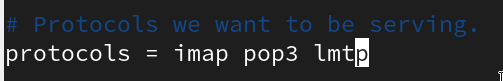
\includegraphics[width=\textwidth]{../images/image01.png}
    \captionof{figure}{Обновление списка разрешенных протоколов в Dovecot.}
    \label{01}
\end{center}
\item Настроили в Dovecot сервис \texttt{lmtp} для связи с Postfix. Для этого в файле \break \texttt{/etc/dovecot/conf.d/10-master.conf} заменили определение сервиса \texttt{lmtp} на следующую запись (Рис. \ref{02}):
  \begin{minted}{bash}
    service lmtp {
      unix_listener /var/spool/postfix/private/dovecot-lmtp {
        group = postfix
        user = postfix
        mode = 0600
      }
    }
  \end{minted}
\begin{center}
    \centering
    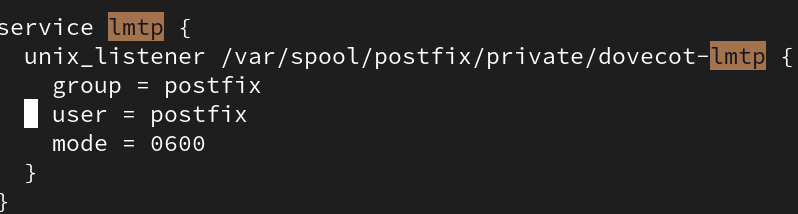
\includegraphics[width=\textwidth]{../images/image02.png}
    \captionof{figure}{Настройки сервера \texttt{lmtp}.}
    \label{02}
\end{center}
%  Эта запись определяет расположение файла с описанием прослушиваемого unix-сокета, а также задаёт права доступа к нему и определяет принадлежность к группе и пользователю postfix.
\item Переопределили в Postfix с помощью \texttt{postconf} передачу сообщений не на прямую, а через заданный unix-сокет:
  \begin{minted}{bash}
    postconf -e 'mailbox_transport = lmtp:unix:private/dovecot-lmtp'
  \end{minted}
\item В файле \texttt{/etc/dovecot/conf.d/10-auth.conf} задали формат имени пользователя для аутентификации в форме логина пользователя без указания домена (Рис. \ref{03}):
  \begin{minted}{bash}
    auth_username_format = %Ln
  \end{minted}
\begin{center}
    \centering
    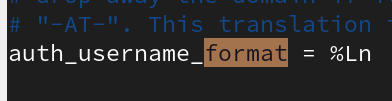
\includegraphics[width=\textwidth]{../images/image03.png}
    \captionof{figure}{Задание формата имени пользователя для аутентификации.}
    \label{03}
\end{center}
\item Перезапустите Postfix и Dovecot (Рис. \ref{04}):
  \begin{minted}{bash}
    systemctl restart postfix
    systemctl restart dovecot
  \end{minted}
\begin{center}
    \centering
    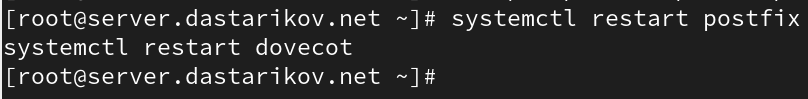
\includegraphics[width=\textwidth]{../images/image04.png}
    \captionof{figure}{Перезагрузка Postfix и Dovecot.}
    \label{04}
\end{center}
\item Из-под учётной записи своего пользователя отправили письмо с клиента:
  \begin{minted}{bash}
    echo .| mail -s "LMTP test" dastarikov@dastarikov.net
  \end{minted}

\item На сервере просмотрели почтовый ящик пользователя  (Рис. \ref{05} и \ref{06}):
  \begin{minted}{bash}
    MAIL=~/Maildir/ mail
  \end{minted}
\begin{center}
    \centering
    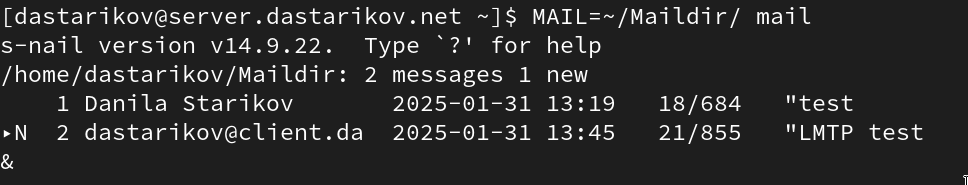
\includegraphics[width=\textwidth]{../images/image05.png}
    \captionof{figure}{Просмотр доставленного письма через утилиту \texttt{mail}.}
    \label{05}
\end{center}
\begin{center}
    \centering
    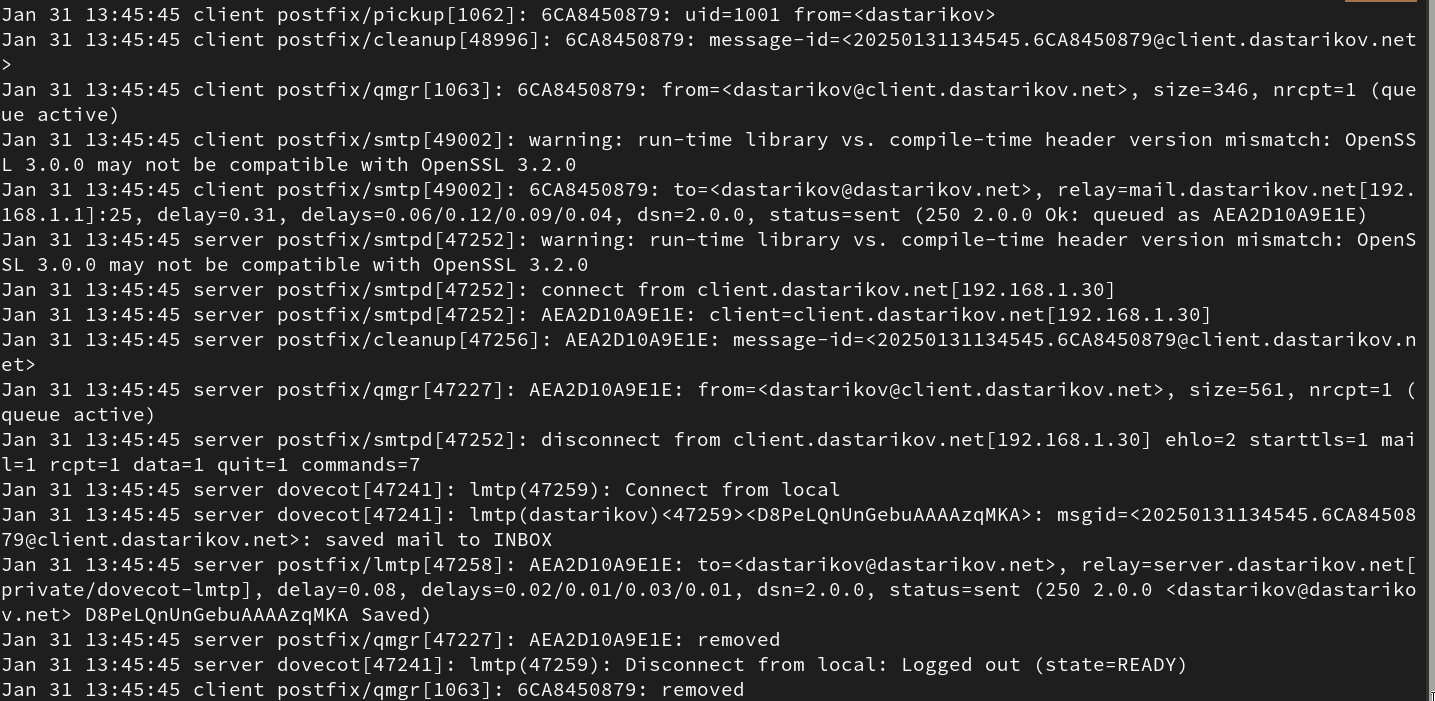
\includegraphics[width=\textwidth]{../images/image06.png}
    \captionof{figure}{Просмотр логов при отправке письма.}
    \label{06}
\end{center}
\end{enumerate}
\subsection{Настройка SMTP-аутентификации}

\begin{enumerate}
\item В файле \texttt{/etc/dovecot/conf.d/10-master.conf} определили службу аутентификации пользователей (Рис. \ref{08}):
  \begin{minted}{bash}
    service auth {
      unix_listener /var/spool/postfix/private/auth {
        group = postfix
        user = postfix
        mode = 0660
      }
      unix_listener auth-userdb {
        mode = 0600
        user = dovecot
      }
    }
  \end{minted}
\begin{center}
    \centering
    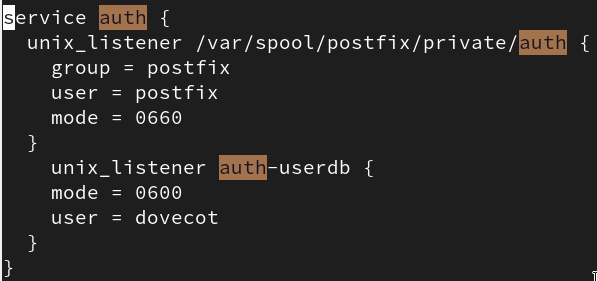
\includegraphics[width=\textwidth]{../images/image08.png}
    \captionof{figure}{Настройка службы аутентификации.}
    \label{08}
\end{center}

\item Для Postfix задали тип аутентификации SASL для \texttt{smtpd} и путь к соответствующему unix-сокету (Рис. \ref{09}):
  \begin{minted}{bash}
    postconf -e 'smtpd_sasl_type = dovecot'
    postconf -e 'smtpd_sasl_path = private/auth'
  \end{minted}
\begin{center}
    \centering
    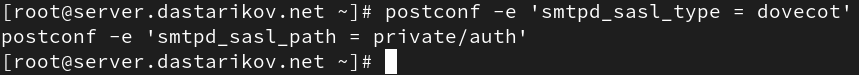
\includegraphics[width=\textwidth]{../images/image09.png}
    \captionof{figure}{Настройка типа аутентификации SASL для \texttt{smtpd}.}
    \label{09}
\end{center}
\item Настроили Postfix для приёма почты из Интернета только для обслуживаемых нашим сервером пользователей или для произвольных пользователей локальной машины (имеется в виду локальных пользователей сервера), обеспечивая тем самым запрет на использование почтового сервера в качестве SMTP relay для спамрассылок (порядок указания опций имеет значение) (Рис. \ref{10}):
  \begin{minted}{bash}
    postconf -e 'smtpd_recipient_restrictions = reject_unknown_recipient_domain, permit_mynetworks, reject_non_fqdn_recipient, reject_unauth_destination, reject_unverified_recipient, permit'
  \end{minted}
\begin{center}
    \centering
    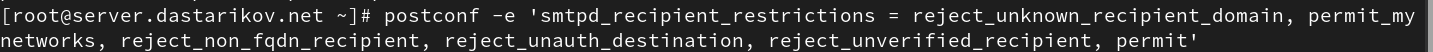
\includegraphics[width=\textwidth]{../images/image10.png}
    \captionof{figure}{Настройка Postfix для запрета спамрассылок.}
    \label{10}
\end{center}

\item В настройках Postfix ограничили приём почты только локальным адресом SMTP-сервера сети (Рис. \ref{11}):
  \begin{minted}{bash}
    postconf -e 'mynetworks = 127.0.0.0/8'
  \end{minted}
\begin{center}
    \centering
    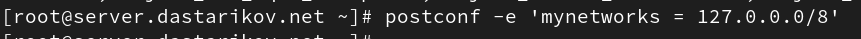
\includegraphics[width=\textwidth]{../images/image11.png}
    \captionof{figure}{Ограничение приема почты только локальным адресом.}
    \label{11}
\end{center}
\item Для проверки работы аутентификации временно запустили SMTP-сервер (порт 25) с возможностью аутентификации. Для этого в файле \texttt{/etc/postfix/master.cf} заменили строку
  \begin{minted}{bash}
    smtp inet n - n - - smtpd
  \end{minted}
  на строку
  \begin{minted}{bash}
    smtp inet n - n - - smtpd
    -o smtpd_sasl_auth_enable=yes
    -o smtpd_recipient_restrictions=reject_non_fqdn_recipient, reject_unknow, n_recipient_domain, permit_sasl_authenticated, reject
  \end{minted}
\item Перезапустили Postfix и Dovecot (Рис. \ref{13}):
  \begin{minted}{bash}
    systemctl restart postfix
    systemctl restart dovecot
  \end{minted}
  \begin{center}
    \centering
    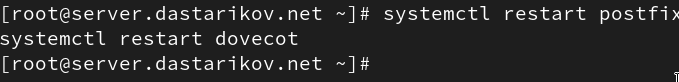
\includegraphics[width=\textwidth]{../images/image13.png}
    \captionof{figure}{Перезагрузка Postfix и Dovecot.}
    \label{13}
\end{center}
\item На клиенте установили \texttt{telnet}:
  \begin{minted}{bash}
    sudo -i
    dnf -y install telnet
  \end{minted}
\item На клиенте получили строку для аутентификации (Рис. \ref{14}):
  \begin{minted}{bash}
    printf 'dastarikov\x00dastarikov\x00123456 | base64
  \end{minted}
\begin{center}
    \centering
    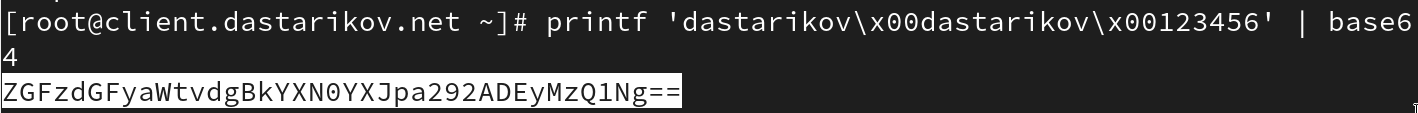
\includegraphics[width=\textwidth]{../images/image14.png}
    \captionof{figure}{Получение строки для аутентификации.}
    \label{14}
\end{center}
\item Подключились на клиенте к SMTP-серверу посредством \texttt{telnet} (Рис. \ref{15}):
  \begin{minted}{bash}
    telnet server.dastarikov.net 25
  \end{minted}
  Протестировали соединение, введя
  \begin{minted}{bash}
    EHLO test
  \end{minted}
  Проверили авторизацию, задав:
  \begin{minted}{bash}
    AUTH PLAIN <строка для аутентификации>
  \end{minted}
\begin{center}
    \centering
    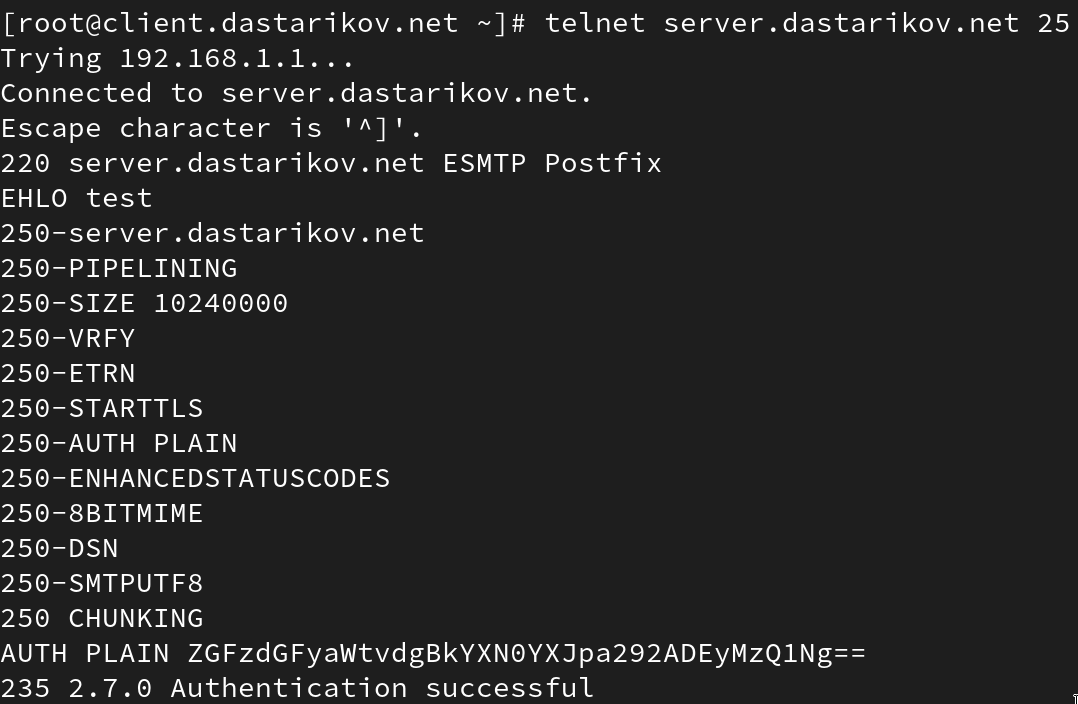
\includegraphics[width=\textwidth]{../images/image15.png}
    \captionof{figure}{Подключение к SMTP-серверу через \texttt{telnet}.}
    \label{15}
\end{center}
  Завершили сессию \texttt{telnet} на клиенте.
\end{enumerate}

\subsection{Настройка SMTP over TLS}

\begin{enumerate}
\item Настроили на сервере TLS, воспользовавшись временным сертификатом Dovecot. Предварительно скопировали необходимые файлы сертификата и ключа из каталога \texttt{/etc/pki/dovecot} в каталог \texttt{/etc/pki/tls/} в соответствующие подкаталоги (чтобы не было проблем с SELinux):
  \begin{minted}{bash}
    cp /etc/pki/dovecot/certs/dovecot.pem /etc/pki/tls/certs
    cp /etc/pki/dovecot/private/dovecot.pem /etc/pki/tls/private
  \end{minted}
  Сконфигурировали Postfix, указав пути к сертификату и ключу, а также к каталогу для хранения TLS-сессий и уровень безопасности (Рис. \ref{16}):
  \begin{minted}{bash}
    postconf -e 'smtpd_tls_cert_file=/etc/pki/tls/certs/dovecot.pem'
    postconf -e 'smtpd_tls_key_file=/etc/pki/tls/private/dovecot.pem'
    postconf -e 'smtpd_tls_session_cache_database = btree:/var/lib/postfix/smtpd_scache'
    postconf -e 'smtpd_tls_security_level = may'
    postconf -e 'smtp_tls_security_level = may'
  \end{minted}
\begin{center}
    \centering
    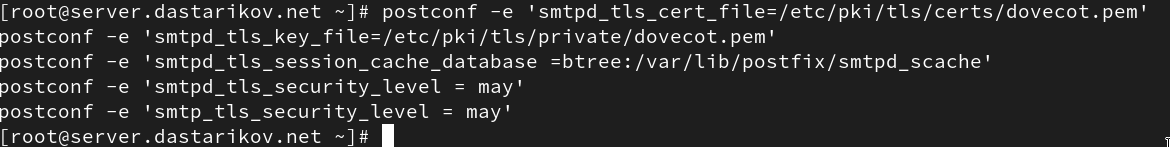
\includegraphics[width=\textwidth]{../images/image16.png}
    \captionof{figure}{Конфигурация Postfix для работы через TLS.}
    \label{16}
\end{center}
\item Для того чтобы запустить SMTP-сервер на 587-м порту, в файле \texttt{/etc/postfix/master.cf} заменили строки (Рис. \ref{17})
  \begin{minted}{bash}
    smtp inet n - n - - smtpd
    -o smtpd_sasl_auth_enable=yes
    -o smtpd_recipient_restrictions=reject_non_fqdn_recipient, reject_unknow, n_recipient_domain, permit_sasl_authenticated, reject
  \end{minted}
  на следующую запись:
  \begin{minted}{bash}
    smtp inet n - n - - smtpd
  \end{minted}
  и добавили следующие строки:
  \begin{minted}{bash}
    submission inet n - n - - smtpd
    -o smtpd_tls_security_level=encrypt
    -o smtpd_sasl_auth_enable=yes
    -o smtpd_recipient_restrictions=reject_non_fqdn_recipient, reject_unknow, n_recipient_domain, permit_sasl_authenticated, reject
  \end{minted}
\begin{center}
    \centering
    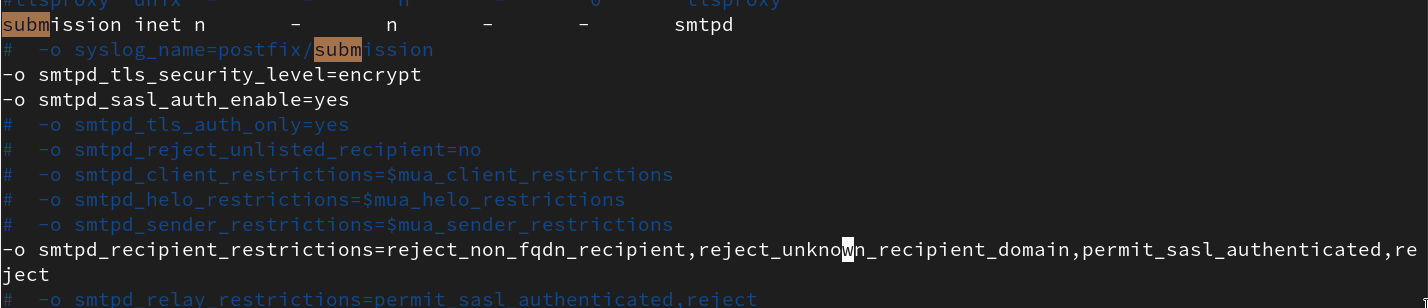
\includegraphics[width=\textwidth]{../images/image17.png}
    \captionof{figure}{Изменение \texttt{/etc/postfix/master/cf}.}
    \label{17}
\end{center}
\item Настроили межсетевой экран, разрешив работать службе \texttt{smtp-submission}:
  \begin{minted}{bash}
    firewall-cmd --get-services
    firewall-cmd --add-service=smtp-submission
    firewall-cmd --add-service=smtp-submission --permanent
    firewall-cmd --reload
  \end{minted}
\item Перезапустили Postfix:
  \begin{minted}{bash}
    systemctl restart postfix
  \end{minted}
\item На клиенте подключились к SMTP-серверу через 587-й порт посредством \texttt{openssl} (вместо dastarikov используйте свой логин) (Рис. \ref{18}):
  \begin{minted}{bash}
    openssl s_client -starttls smtp -crlf -connect server.dastarikov.net:587
  \end{minted}
\begin{center}
    \centering
    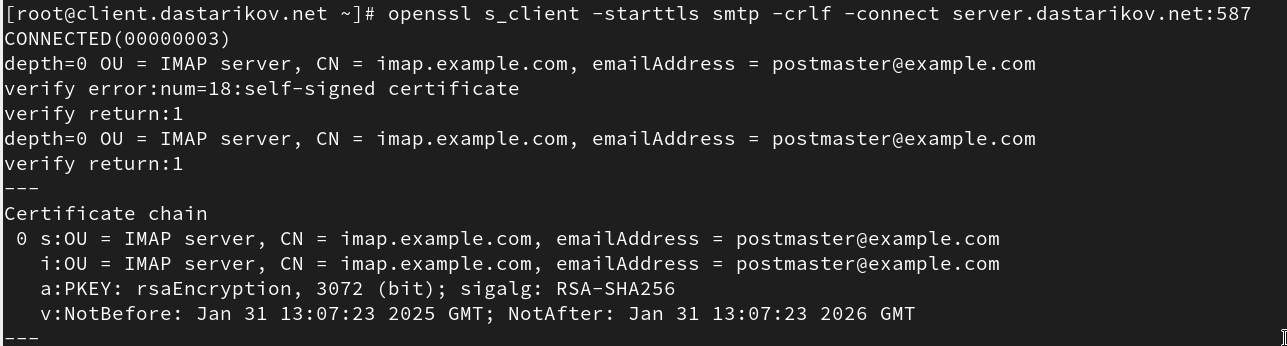
\includegraphics[width=\textwidth]{../images/image18.png}
    \captionof{figure}{Подключение к SMTP-серверу через \texttt{openssl}.}
    \label{18}
\end{center}

  Протестировали подключение по \texttt{telnet} (Рис. \ref{19}):
  \begin{minted}{bash}
    EHLO test
  \end{minted}
  Проверили аутентификацию (Рис. \ref{19}):
  \begin{minted}{bash}
    AUTH PLAIN <строка для аутентификации>
  \end{minted}
\begin{center}
    \centering
    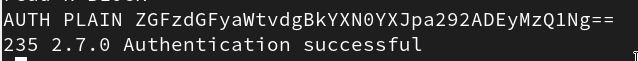
\includegraphics[width=\textwidth]{../images/image19.png}
    \captionof{figure}{Проверка подключения к SMTP-серверу через \texttt{telnet}.}
    \label{19}
\end{center}
\item Проверили корректность отправки почтовых сообщений с клиента посредством почтового клиента Evolution, предварительно скорректировав настройки учётной записи, а именно для SMTP-сервера указали порт 587, STARTTLS и обычный пароль (Рис. \ref{20}-\ref{22}).
\begin{center}
    \centering
    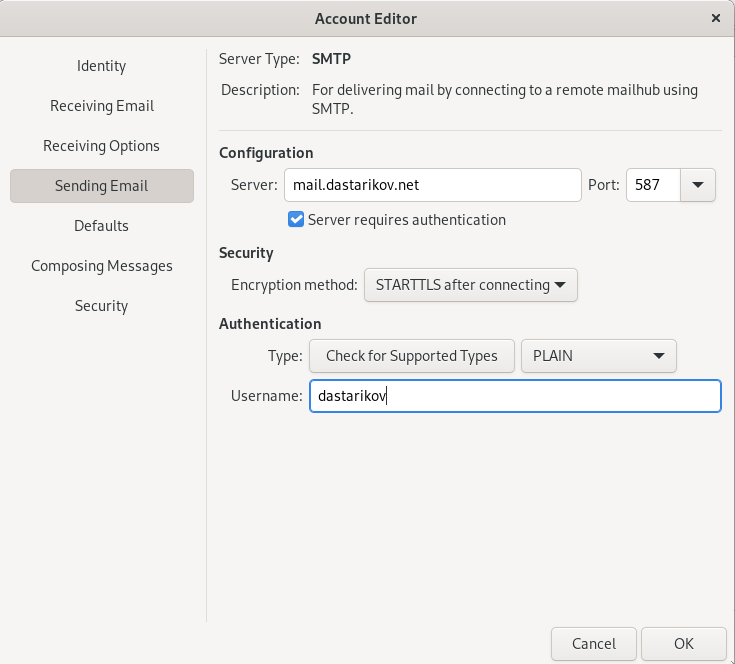
\includegraphics[width=\textwidth]{../images/image20.png}
    \captionof{figure}{Корректировка почтового клиента Evolution.}
    \label{20}
\end{center}
\begin{center}
    \centering
    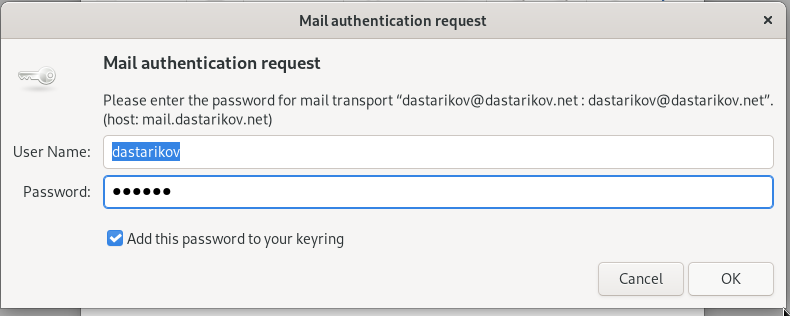
\includegraphics[width=\textwidth]{../images/image21.png}
    \captionof{figure}{Аутентификация пользователя при попытке отправить письмо.}
    \label{21}
  \end{center}
  \begin{center}
    \centering
    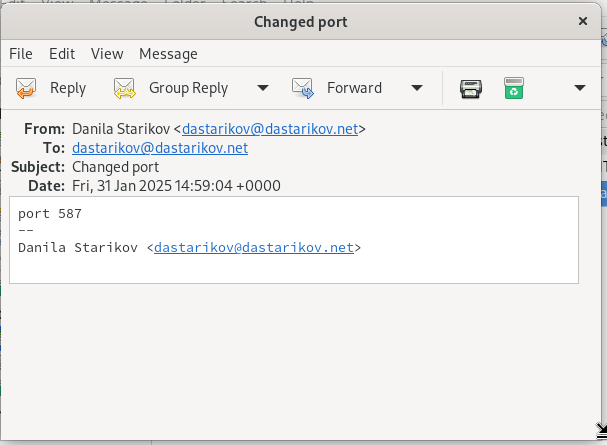
\includegraphics[width=\textwidth]{../images/image22.png}
    \captionof{figure}{Просмотр пришедшего письма.}
    \label{22}
\end{center}
\end{enumerate}

\subsection{Внесение изменений в настройки внутреннего окружения виртуальной машины}

\begin{enumerate}
\item На виртуальной машине \texttt{server} перешли в каталог для внесения изменений в настройки внутреннего окружения \texttt{/vagrant/provision/server/}. В соответствующие подкаталоги поместили конфигурационные файлы Dovecot и Postfix:
  \begin{minted}{bash}
    cd /vagrant/provision/server
    cp -R /etc/dovecot/dovecot.conf /vagrant/provision/server/mail/etc/dovecot/
    cp -R /etc/dovecot/conf.d/10-master.conf /vagrant/provision/server/mail/etc/dovecot/conf.d/
    cp -R /etc/dovecot/conf.d/10-auth.conf /vagrant/provision/server/mail/etc/dovecot/conf.d/
    mkdir -p /vagrant/provision/server/mail/etc/postfix/
    cp -R /etc/postfix/master.cf /vagrant/provision/server/mail/etc/postfix/
  \end{minted}
\item Внесли соответствующие изменения по расширенной конфигурации SMTP-сервера в файл \texttt{/vagrant/provision/server/mail.sh}:
  \begin{minted}{bash}
    #!/bin/bash
    echo "Provisioning script $0"
    echo "Install needed packages"
    dnf -y install postfix
    dnf -y install dovecot
    dnf -y install telnet
    echo "Copy configuration files"
    cp -R /vagrant/provision/server/mail/etc/* /etc
    chown -R root:root /etc/postfix
    restorecon -vR /etc
    echo "Configure firewall"
    firewall-cmd --add-service smtp --permanent
    firewall-cmd --add-service pop3 --permanent
    firewall-cmd --add-service pop3s --permanent
    firewall-cmd --add-service imap --permanent
    firewall-cmd --add-service imaps --permanent
    firewall-cmd --add-service smtp-submission --permanent
    firewall-cmd --reload
    echo "Start postfix service"
    systemctl enable postfix
    systemctl start postfix
    echo "Configure postfix"
    postconf -e 'mydomain = dastarikov.net'
    postconf -e 'myorigin = $mydomain'
    postconf -e 'inet_protocols = ipv4'
    postconf -e 'inet_interfaces = all'
    postconf -e 'mydestination = $myhostname, localhost.$mydomain, localhost, $mydomain'
    #postconf -e 'mynetworks = 127.0.0.0/8, 192.168.0.0/16'
    echo "Configure postfix for dovecot"
    postconf -e 'home_mailbox = Maildir/'
    echo "Configure postfix for auth"
    postconf -e 'smtpd_sasl_type = dovecot'
    postconf -e 'smtpd_sasl_path = private/auth'
    postconf -e 'smtpd_recipient_restrictions = reject_unknown_recipient_domain, permit_mynetworks, reject_non_fqdn_recipient, reject_unauth_destination, reject_unverified_recipient, permit'
    
    postconf -e 'mynetworks = 127.0.0.0/8'
    echo "Configure postfix for SMTP over TLS"
    cp /etc/pki/dovecot/certs/dovecot.pem /etc/pki/tls/certs
    cp /etc/pki/dovecot/private/dovecot.pem /etc/pki/tls/private
    postconf -e 'smtpd_tls_cert_file=/etc/pki/tls/certs/dovecot.pem'
    postconf -e 'smtpd_tls_key_file=/etc/pki/tls/private/dovecot.pem'
    postconf -e 'smtpd_tls_session_cache_database = btree:/var/lib/postfix/smtpd_scache'
    postconf -e 'smtpd_tls_security_level = may'
    postconf -e 'smtp_tls_security_level = may'
    postfix set-permissions
    restorecon -vR /etc
    systemctl stop postfix
    systemctl start postfix
    systemctl restart dovecot
  \end{minted}
\item Внесли изменения в файл \texttt{/vagrant/provision/client/mail.sh}, добавив установку \texttt{Telnet}.
  \begin{minted}{bash}
    dnf -y install telnet
  \end{minted}
\end{enumerate}

\section{Выводы}
В результате выполнения лабораторной работы приобрели практические навыки по конфигурированию SMTP-сервера в части настройки аутентификации.
\end{document}
